\chapter{Colouring}\label{chpt:colouring}

\section{Introduction}

Long ago all world maps were hand drawn. Alice has a business that specializes in drawing world maps. Each map is beautifully hand coloured. Each country getting its own colour. To ensure the maps are visually appealing and to help distinguish countries no two bordering countries can be the same colour. In those days ink was expensive. So Alice wishes to use the least number of colours possible. What is the smallest number of colours Alice needs to colour a map in such a fashion? 

\begin{figure}[h]
    \centering
    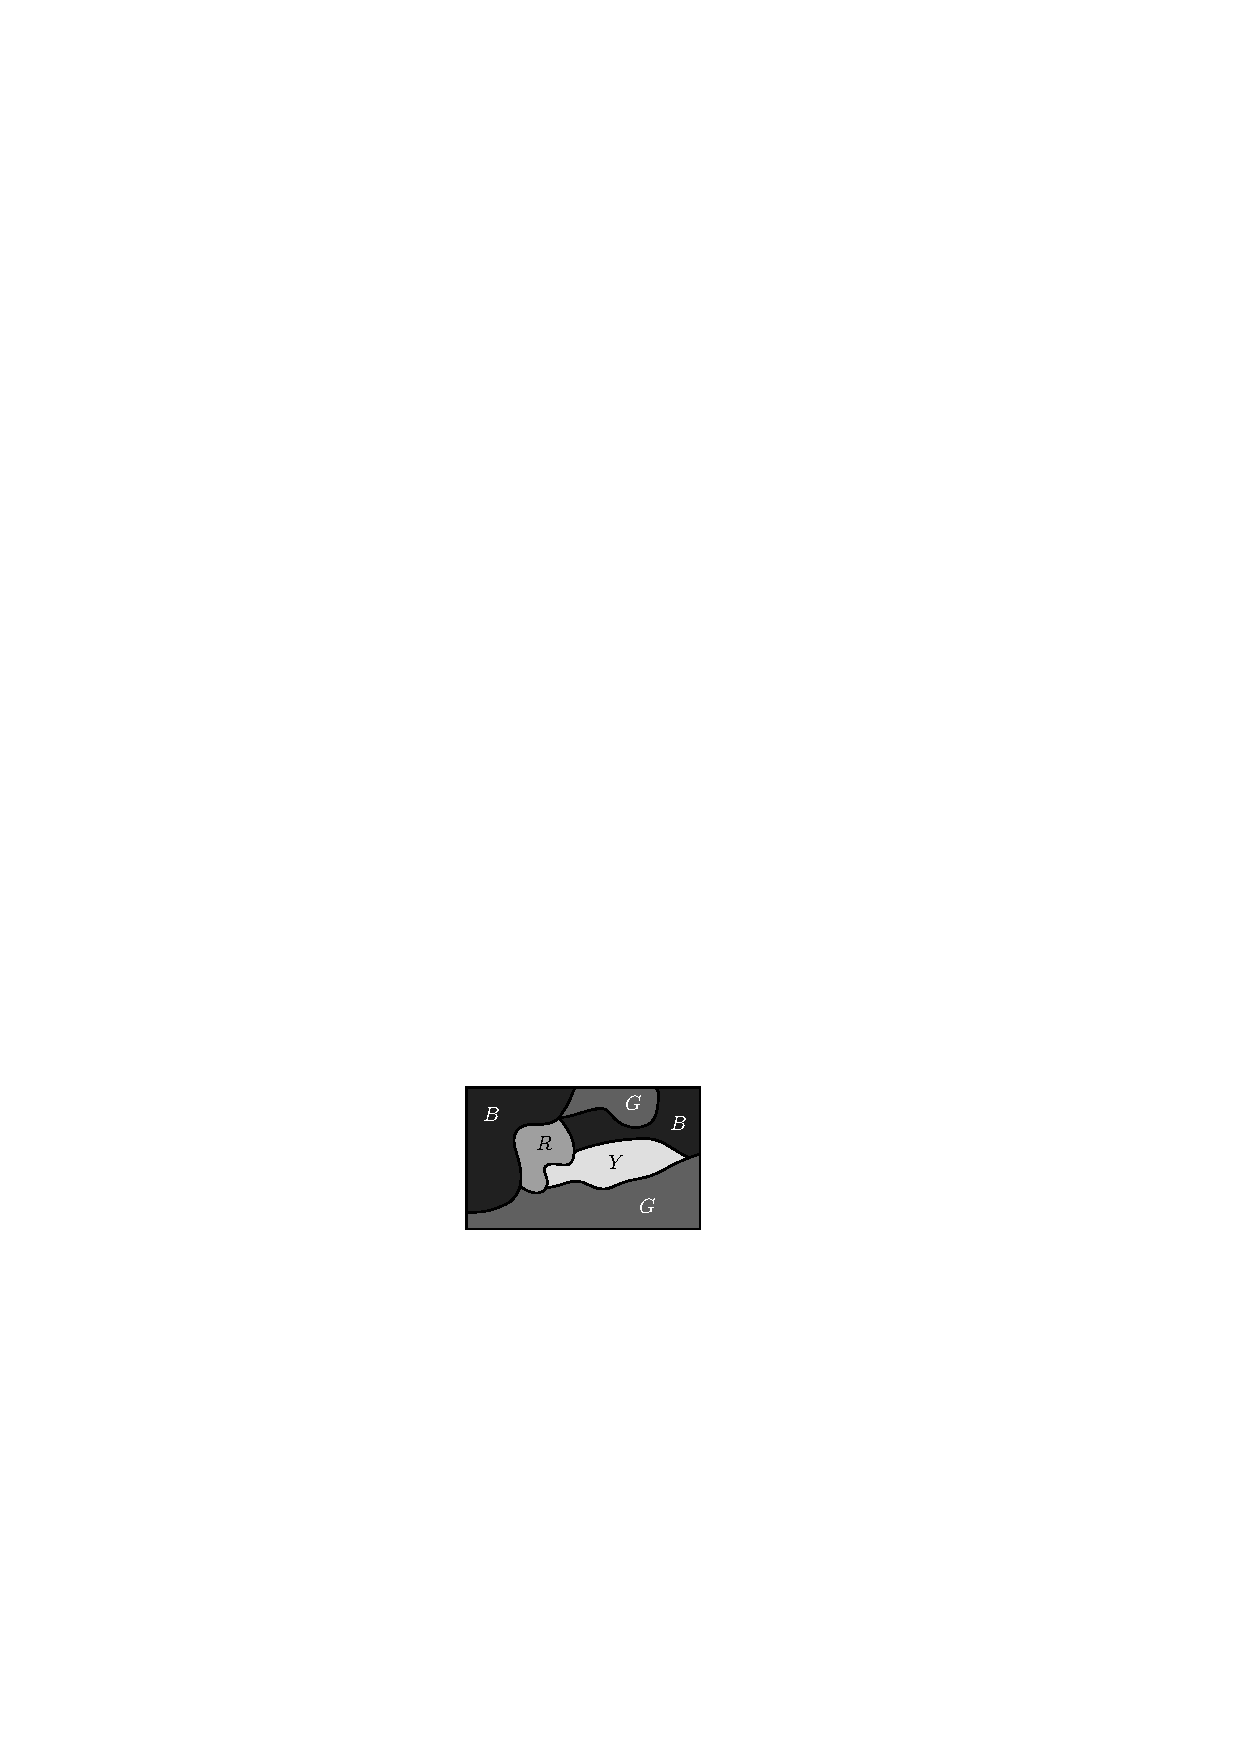
\includegraphics[height=40mm]{images/161-fig37}
    \caption{A coloured map}
\end{figure}

We can translate the problem of map colouring to a problem about graphs. We do this by placing a vertex in each country and join two vertices with an edge if and only if the corresponding countries share a border. 
\begin{figure}[h]
    \centering
    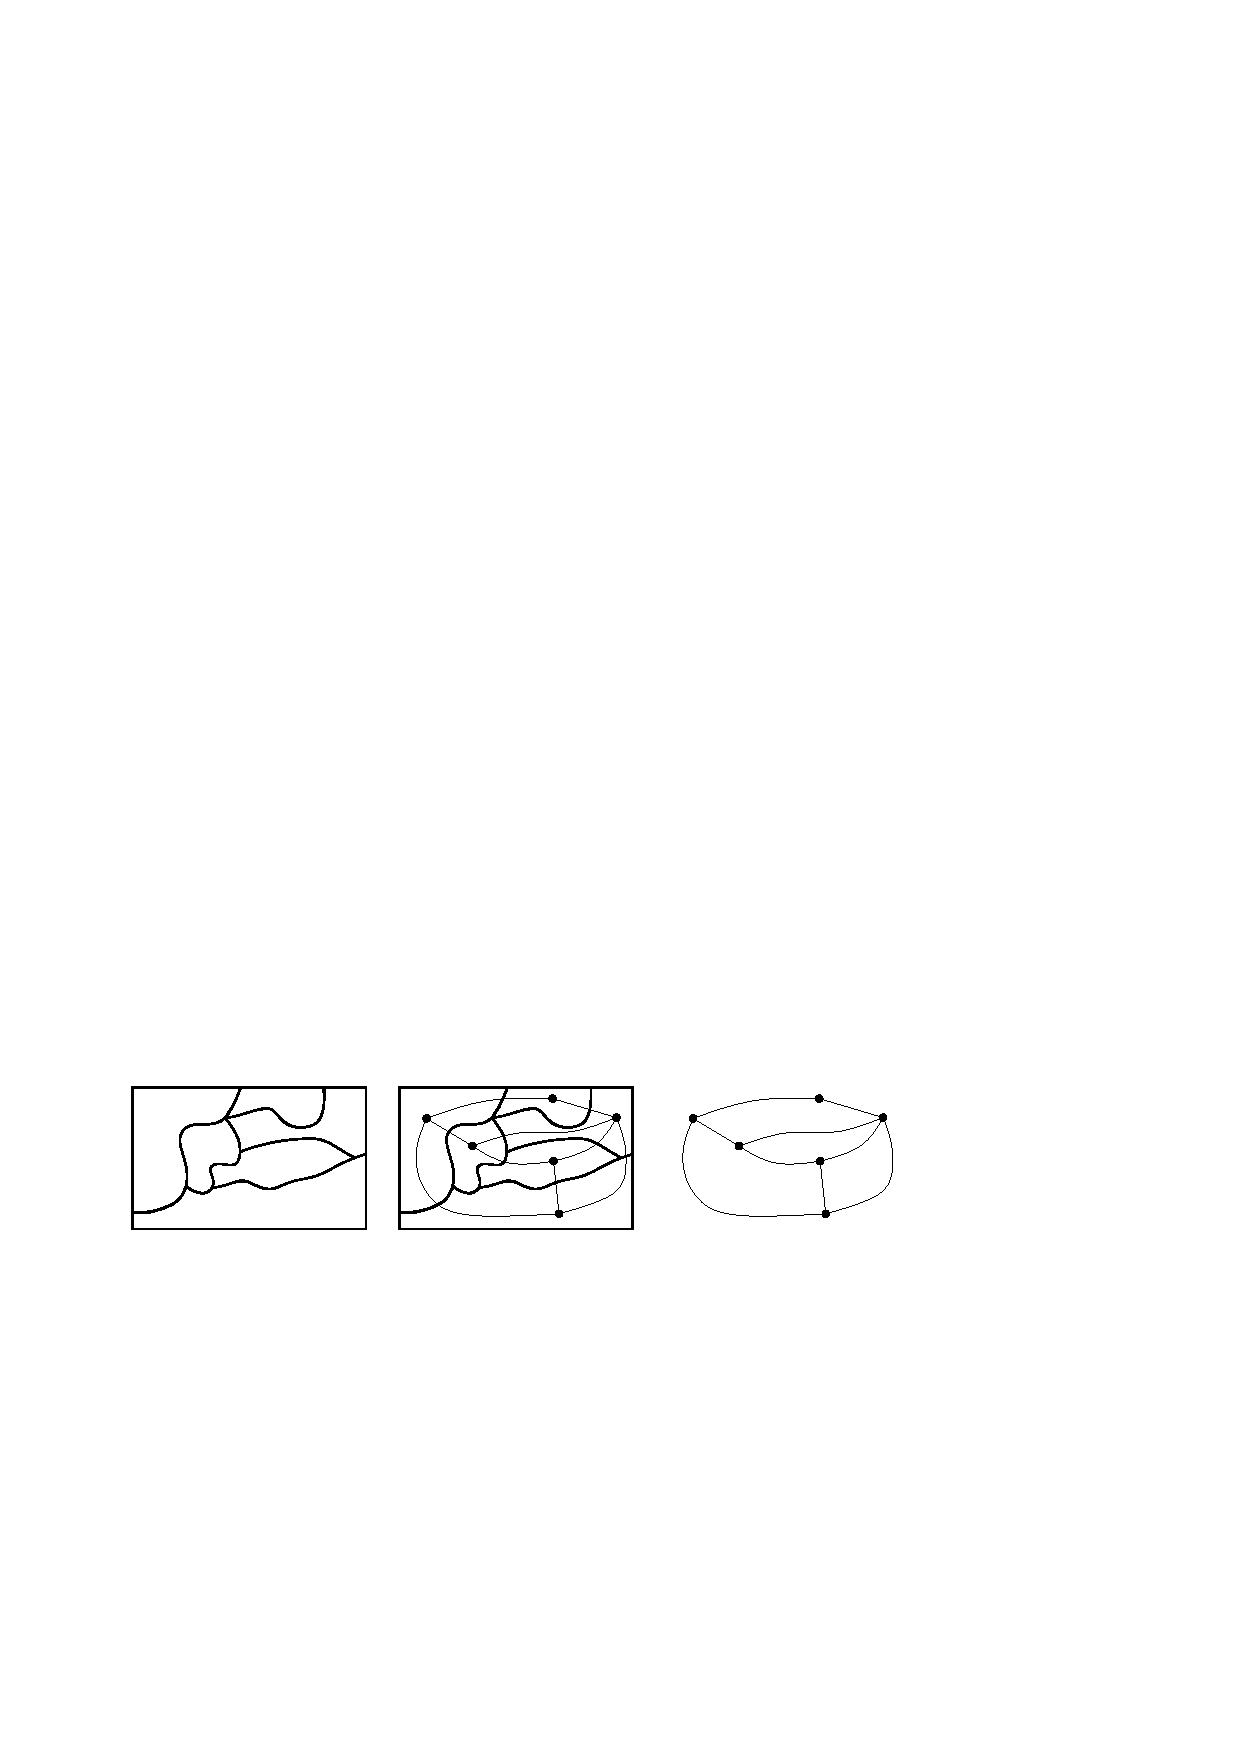
\includegraphics[width=\textwidth]{images/161-fig38}
    \caption{Translating maps to graphs}
\end{figure}
By constructing a graph in this way be have a one to one correspondence between colourings of the graph and the map. So, if Alice assign colours to the vertices such that no two neighbouring vertices have the same colour She has a way to colour the map. Any graph that can be drawn on the plane can be coloured in this manor using only four colours. This is known as the \textit{four colour theorem} \cite{thomas19984ColourUpdate}. The four colour theorem states that any planar graph can be coloured using only four colours. Thus Alice needs only 4 colours to colour her maps.

We formally define a colouring as follows.
\begin{definition}[Proper $k$--Vertex Colouring]
Let $C=\{1,\dots,k\}$ be a set of colours, a $k$--vertex colouring of a graph $G$ is a mapping $c\colon V(G) \to C$. A \textit{proper $k$--vertex colouring} of $G$ is a mapping $c\colon V(G) \to C$ such that for two vertices $u,v\in V(G)$ if $(u,v)\in E(G)$ then $c(u)\neq c(v)$. 
\end{definition}
When referring to graph colourings we will henceforth be referring to proper $k$--vertex colourings for some $k$. 
\begin{definition}[Chromatic Number]
The \textit{chromatic number}, $\chi(G)$, of a graph $G$ is the smallest $k$ such that $G$ has a proper $k$--vertex colouring.
\end{definition} 

\section{The Colouring Game} \label{sec:colouring_game}
Alice's map colouring businesses is a huge success. She decides to hire Bob to help her colour maps. Unbeknownst to Alice Bob is part of a secret ink cabal. The cabal's sole goal is to drive up ink sales. Bob will try to use as many colours as possible when colouring maps. To colour a map Alice and Bob take turns assigning a colour to each country. They continue until all the countries are coloured. A problem arises almost immediately. By strategical choosing colours Bob can make it so that some maps \textit{cannot} be coloured with four colours. In fact for some maps Bob can force 8 colours \cite{kierstead1994planar}. So, what is the total number of colours Alice needs to ensure that any map can always be coloured? This is an open question. The current best bound is 17 \cite{Zhu2008}. In section \ref{sec:refActStrat} we will show how this bound is found. We can also ask the same question about classes of graphs other than planer ones. 

But first we define the \textit{colouring game}. Let $G$ be a graph, and $C$ a set of colours. Beginning with Alice, Alice and Bob take alternating turns. On their turn they choose an uncoloured vertex, $v$, and assign $v$ a colour from $C$ such that no two adjacent vertices in $G$ have the same colour. This continues until one of two win conditions are meet. First, Alice wins if all the vertices are coloured. Second, Bob wins if there is a vertex that cannot be coloured with the available colours.

%todo prove subgraphs are bounded by the parent

\begin{definition}[Game Chromatic Number]
    For a graph $G$ the \textit{game chromatic number}, $\chi_g(G)$, is the smallest number of colours needed to guarantee that Alice has a winning strategy on $G$, when playing the colouring game in $G$.     
\end{definition}

Consider a graph $G$. If there is a winning strategy for Bob with $n$ colours then $n+1$ is a lower bound for the game chromatic number of $G$. That is $n\leq\chi_g(G)$. Conversely, if there is a strategy for Alice that guarantees a colouring with $m$ colours then $m$ is an upper bound for the game chromatic number, that is $\chi_g(G)\leq m$.

\subsection{Lower bounds for the $(a,b)$--colouring game}

We consider an extension of the colouring game, the $(a,b)$--colouring game. In the $(a,b)$--colouring game the win conditions and rules are the same as the standard game. But on each turn Alice colours $a$ vertices and Bob colours $b$ turns.
\begin{definition}[$(a,b)$--Game Chromatic Number]
    Let $G$ be a graph, and $a,b\in\mathbb{N}$. 
    Then, $\chi_g(G;a,b)$ is the smallest number of colours needed to guarantee that Alice has a winning strategy on $G$, when playing the $(a,b)$--colouring game. 
\end{definition}
Note that $\chi_g(G) = \chi_g(G;1,1)$.

The first results we will look at are some lower bounds for the game chromatic number.


Bodlaender 1990 \cite{bodlander1990} showed that for the class of trees $\TT$,  $\chi_g(\TT) \geq 4$. He did it by defining a tree and an associated strategy for Bob. We take this proof and extend it to a new proof of theorem \ref{thm:treeColLow}. 

\begin{theorem}\label{thm:treeColLow} %todo reference
    Let $\TT$ be the class of trees. If we have $b \geq 1$  then,
    \[\chi_g(\TT;1,b) \geq b+3 \]
\end{theorem}

\begin{proof}[Proof (Askes)]
    It suffices to show that there exists a tree in which Bob has a winning strategy with $b+2$ colours.
    
    Consider the tree $T$ as defined in figure \ref{fig:multiPlayerTree1}. 
          
   \begin{figure}[h]
       \centering
        \begin{tikzpicture}[scale=.9, transform shape]
        \node [normal] (v7) at (-7.5,1) {};
        \node [normal] (v6) at (-11,1) {};
        \node [normal] (v5) at (-14.5,1) {};
        \node [normal] (v2) at (-18.5,1) {};
        \node [normal] (v1) at (-21,1) {};
        \node [normal] (v3) at (-19,-1) {};
        \node [normal] (v4) at (-17,-1) {};
        \node [normal] (v11) at (-15,-1) {};
        \node [normal] (v10) at (-13.5,-1) {};
        \node [normal] (v9) at (-11.5,-1) {};
        \node [normal] (v8) at (-10,-1) {};
        \node [normal] (v15) at (-9,-1) {};
        \node [normal] (v16) at (-8,-1) {};
        \node [normal] (v17) at (-6.5,-1) {};
        \node [normal] (v12) at (-20,-1) {};
        \node [normal] (v13) at (-16,-1) {};
        \node [normal] (v14) at (-12.5,-1) {};
        \node [normal] (v18) at (-5,1) {};
        \draw  (v1) edge (v2);
        \draw  (v1) edge (v2);
        \draw  (v2) edge (v3);
        \draw  (v2) edge (v4);
        \draw  (v2) edge (v5);
        \draw  (v5) edge (v6);
        \draw  (v6) edge (v7);
        \draw  (v6) edge (v8);
        \draw  (v6) edge (v9);
        \draw  (v5) edge (v11);
        \draw  (v5) edge (v10);
        \draw  (v2) edge (v12);
        \draw  (v13) edge (v5);
        \draw  (v14) edge (v6);
        \draw  (v15) edge (v7);
        \draw  (v16) edge (v7);
        \draw  (v7) edge (v17);
        \draw  (v7) edge (v18);
        \node at ($(v3)!.5!(v4)$) {\ldots};
        \node at ($(v3)!.5!(v4)$) {\ldots};
        \node at ($(v11)!.5!(v10)$) {\ldots};
        \node at ($(v9)!.5!(v8)$) {\ldots};
        \node at ($(v16)!.5!(v17)$) {\ldots};
        
%        \draw [decorate,decoration={calligraphic brace,amplitude=11pt,mirror,raise=2ex}, line width=1.5pt]
%        (v12) -- (v4) node[midway,yshift=-3em]{$p$ vertices};
        \draw[decorate, decoration={brace, amplitude=10pt,mirror,raise=2ex}, thick] ($(v12)+(-.25,0)$)--($(v4)+(.25,0)$) node[midway,yshift=-3em]{$b+1$ vertices};
        \end{tikzpicture}
        \caption{A tree, $T$}
        \label{fig:multiPlayerTree1}
    \end{figure}    
    
    Let $\{c_1,c_2,\ldots,c_{b+1},c_{b+2}\}$ be the set of available colours.
    On Alice's first move she plays any vertex, $v$, and colours it. Let the colour of $v$ be $c_1$.
    Bobs first move is to colour any vertex with distance 3 to $v$. We now have a subgraph in $T$ of the type shown in figure \ref{fig:subgraphColouring}. Bob then colours $y_1, \dots, y_{b-1}$ with $c_2, \dots, c_{b}$ respectively.
\begin{figure}[H]
    \centering
    \begin{tikzpicture}[scale=1,transform shape]
    \tikzstyle{every node}=[circle]; 
    \node [label=above left:4, normalBlack, label=below right:{\footnotesize$c_1$}] (v6) at (-11.5,1) {};
    \node [label=above left:3, normal] (v5) at (-14.5,1) {};
    \node [label=above left:2, normal] (v2) at (-19.5,1) {};
    \node [label=above left:1, normalBlack, label=below right:{\footnotesize$c_1$}] (v1) at (-22,1) {};
    \node [label=below:$x_1$, normal] (v12) at (-21,-1) {};
    \node [label=below:$x_2$, normal] (v3) at (-20,-1) {};
    \node [label=below:$x_{b+1}$, normal] (v4) at (-18.5,-1) {};
    \node [label=below:$y_1$, normalBlack, label=above left:{\footnotesize$c_2$}] (v13) at (-16.5,-1) {};
    \node [label=below:$y_2$, normalBlack, label=above left:{\footnotesize$c_3$}] (v11) at (-15.5,-1) {};
    \node [label=below:$y_{b-1}$, normalBlack, label=above left:{\footnotesize$c_{b}$}] (v10) at (-14,-1) {};
    \node [label=below:$y_{b}$,normal] (v7) at (-13,-1) {};
    \node [label=below:$y_{b+1}$,normal] (v8) at (-12,-1) {};
    \draw  (v1) edge (v2);
    \draw  (v2) edge (v3);
    \draw  (v2) edge (v4);
    \draw  (v2) edge (v5);
    \draw  (v5) edge (v6);
    \draw  (v5) edge (v11);
    \draw  (v5) edge (v10);
    \draw  (v2) edge (v12);
    \draw  (v13) edge (v5);   
    \draw  (v5) edge (v7);
    \draw  (v5) edge (v8);
    \node (e1) at ($(v3)!.5!(v4)$) {\ldots};
    \node (e1) at ($(v11)!.5!(v10)$) {\ldots};
    \end{tikzpicture}
    \caption{A subgraph of the tree $T$ in figure \ref{fig:multiPlayerTree1}}
    \label{fig:subgraphColouring}
\end{figure}

    We consider three cases.
    
    \begin{enumerate}
        \item Alice colours $2$, $x_1$, $x_2$, \ldots, or $x_{b+1}$.
        
        Bob colours $y_{b}$ with $c_{b+1}$ and $y_{b+1}$ with $c_{b+2}$. 
        Vertex $3$ now has $b+2$ different coloured neighbours and therefore Bob wins.     
                    
        \item Alice colours $3$.
               
        The colour of $3$ cannot be one of $c_1 \ldots c_{b}$. Therefore $3$ is either coloured $c_{b+1}$ or $c_{b+2}$. 
        Without loss of generality assume the colour of $3$ is $c_{b+2}$.
        Bob colours $x_1, \dots ,x_{b}$ with $c_2,\dots,c_{b+1}$ respectively.
        Vertex $2$ now has $b+2$ different coloured neighbours and therefore Bob wins.  
                       
        \item Alice colours $y_{b}$ or $y_{b+1}$
        
        Bob colours $2$ with $c_{b+1}$ and $y_{b+1}$ (or $y_{b}$ if Alice coloured $y_{b+1}$) with $c_{b+2}$ .
        Vertex $2$ now has $b+2$ different coloured neighbours and therefore Bob wins. 
    \end{enumerate}

    Therefore we have a winning strategy on $G \in\TT$ for Bob with $b+2$ colours. 
\end{proof}

\subsubsection{Graphs of bounded Pathwidth}

We will now temporally set aside trees and look at graphs of bounded pathwidth. The pathwidth of a graph can be considered a measure of how "path like" a graph is. 
\begin{figure} [h]
    \centering
    \begin{minipage}{.45\textwidth}
        \centering
        \begin{tikzpicture}[scale=1]
        \node [normal, label=left:$a$] (v1) at (0,0) {};
        \node [normal, label=below left:$b$] (v3) at (0,1) {};
        \node [normal, label=left:$c$] (v9) at (0,2) {};
        \node [normal, label=left:$d$] (v4) at (-1.5,0) {};
        \node [normal, label=left:$e$] (v2) at (-2,1) {};
        \node [normal, label=left:$f$] (v5) at (1.5,0) {};
        \node [normal, label=below left:$g$] (v6) at (2,1) {};
        \draw [] (v2) edge (v3);
        \draw [] (v3) edge (v4);
        \draw [] (v3) edge (v5);
        \draw [] (v6) edge (v3);
        \draw [] (v1) edge (v3);
        \node [normal, label=below left:$h$] (v10) at (1,2) {};
        \node [normal, label=left:$i$] (v11) at (1,3) {};
        \node [normal, label=left:$j$] (v12) at (2,3) {};
        \draw [] (v9) edge (v10);
        \draw [] (v10) edge (v11);
        \draw [] (v10) edge (v12);
        \draw [] (v9) edge (v3);
        \end{tikzpicture}
        \caption{A graph of pathwidth 1}
        \label{fig:pathwidth1}
    \end{minipage}
    \begin{minipage}{.45\textwidth}
        \centering
        \begin{tikzpicture}[scale=.8]
        \node [normal,label = left:$a$] (v4) at (-4,-2) {};
        \node [normal,label = left:$b$] (v1) at (-4,0) {};
        \node [normal,label = above left:$c$] (v2) at (-2,0) {};
        \node [normal,label = below left:$d$] (v3) at (-2,-2) {};
        \node [normal,label = above left:$e$] (v5) at (0,0) {};
        \node [normal,label = left:$f$] (v6) at (0.2,-0.9) {};
        \node [normal,label = below:$g$] (v7) at (1.3,-1.4) {};
        \node [normal,label = above left:$h$] (v8) at (3,0) {};
        \node [normal,label = below left:$i$] (v9) at (2,-3) {};
        \draw  (v1) edge (v2);
        \draw  (v2) edge (v3);
        \draw  (v3) edge (v4);
        \draw  (v4) edge (v1);
        \draw  (v2) edge (v5);
        \draw  (v5) edge (v3);
        \draw  (v3) edge (v6);
        \draw  (v6) edge (v5);
        \draw  (v6) edge (v7);
        \draw  (v5) edge (v8);
        \draw  (v8) edge (v7);
        \draw  (v7) edge (v9);
        \draw  (v9) edge (v8);
        \draw  (v9) edge (v3);
        \draw  (v7) edge (v3);
        \draw  (v1) edge (v3);
        \draw  (v4) edge (v2);
        \end{tikzpicture}
        \caption{A graph of pathwidth 3}
        \label{fig:pathwidth2}
    \end{minipage}
\end{figure} 
For example, the graphs of path width 1 are caterpillars and unions of caterpillars, such graphs are almost paths (see figure \ref{fig:pathwidth1}). Figure \ref{fig:pathwidth2} is a graph of pathwidth 3 and is noticeably less path like. 

\begin{definition}[Path Decomposition]
    Let $G$ be a graph. A \textit{path decomposition} is set of subsets of $V(G)$, $P=(P_1,P_2,\dots,P_n)$ such that $\bigcup_{i} P_i=V(G)$ and has the following properties.    
    \begin{enumerate}[(i)]
        \item For all edges $(u,v) \in E(G)$ there exists an $i$ such that such $u,v\in P_i$
        \item If there exists an $i\leq j$ and vertices $u,v$ such that $v\in P_i$ and, $v\in P_j$ then for all $i<k<j$, $v\in P_k$
    \end{enumerate}
    The width of a path decomposition is one less the size if the largest set in $P$.
\end{definition}

\begin{definition}[Pathwidth]
    The pathwidth of a graph $G$ is the minimum width of a path decomposition of $G$.    
    A graph of bounded pathwidth, $k$, is a graph with a pathwidth less than or equal to $k$. 
\end{definition}

As an example consider the graphs is figures \ref{fig:pathwidth1} and \ref{fig:pathwidth2}. The graph in figure \ref{fig:pathwidth1} has pathwidth 1 and the path decomposition
\[(\{a,b\},\{b,d\},\{b,e\},\{b,a\},\{b,f\},\{b,f\},\{b,c\},\{c,h\},\{h,i\},\{h,j\})\]
And the graph in figure \ref{fig:pathwidth2} has pathwidth 3 and the path decomposition 
\[(\{a,b,c,d\},\{c,d,e\},\{e,c,f,g\},\{e,d,g,h\},\{d,g,h,i\})\] 

A maximal graph, $G$, of pathwidth $k$ is a graph that we cannot add any more edges to $G$ without increasing its pathwidth. In such a graph every element in its path decomposition is a $(k+1)$--clique. These graphs are known as \textit{$k$--paths}.
\begin{definition}[$k$--path]
    A \textit{$k$--path} is a maximal graph of pathwidth $k$.
\end{definition}

\begin{figure}[h]
    \centering
    \begin{tikzpicture}
    \node [normal,label = left:$ $] (v4) at (-4,-2) {};
    \node [normal,label = left:$ $] (v1) at (-4,0) {};
    \node [normal,label = above left:$ $] (v2) at (-2,-1) {};
    \node [normal,label = left:$ $] (v3) at (-3,-1) {};
    \node [normal,label = below left:$ $] (v5) at (-2,1) {};
    \node [normal,label = below left:$ $] (v6) at (-0.6,-1.5) {};
    \node [normal,label = above left:$ $] (v7) at (-1,1) {};
    \node [normal,label = below:$ $] (v8) at (1,0) {};
    
    \draw  (v1) edge (v2);
    \draw  (v2) edge (v3);
    \draw  (v3) edge (v4);
    \draw  (v4) edge (v1);
    \draw  (v1) edge (v3);
    \draw  (v4) edge (v2);
    \draw  (v1) edge (v5);
    \draw  (v5) edge (v3);
    \draw  (v2) edge (v5);
    \draw  (v6) edge (v2);
    \draw  (v3) edge (v6);
    \draw  (v6) edge (v5);
    \draw  (v3) edge (v7);
    \draw  (v7) edge (v5);
    \draw  (v7) edge (v6);
    \draw  (v3) edge (v8);
    \draw  (v6) edge (v8);
    \draw  (v8) edge (v7);
    \end{tikzpicture}
    \caption{A $k$--path with width 3}
\end{figure}

 A $k$--path $G$ contains a $k+1$ clique and so there is no proper colouring with less than $k+1$ colours. Hence, when playing the colouring game on a $k$--path Bob will always win if there are $k$ or less colours. 
 \begin{theorem}
 For $G$ a $k$--path,
    \[k < \chi_g(G) \] 
 \end{theorem}

\begin{theorem}[Fragile, Kern, Kierstead, Trotter 1993 \cite{faKeKiTr1993}]
    Let $\PP_k$ be class of graphs with bounded pathwidth $k$. If we have $b\geq1$  then \[(b+1)k+\left\lceil \frac{b}{2}\right\rceil\leq\chi_g(\PP_k;1,b)\]
\end{theorem}

This result first apearied in Fragile, Kern, Kierstead, Trotter 1993 \cite{faKeKiTr1993} as a lower bound for the $(1,1)$--colouring game. In \cite{faKeKiTr1993} the authors do not give a formal proof, they inspire a proof. This is something we aim to remedy in this report. We do this by proving a new proof. At the same time we  extend the ideas to the $(1,b)$--colouring game.
\begin{proof}
    It suffices to show that there exists a graph in $\PP_k$ for which Bob has a winning strategy with $m=(b+1)k+\left\lceil\frac{b}{2}\right\rceil-1$ colours. Let the set of available colours be $C=\{c_1,c_2,\dots,c_m\}$.
    
    We define the graph $G$ as follows. Start with a $k$-clique, $K_k$, then take $n=2|C|+1$ vertices, $v_1,\dots,v_n$ and connect each $v_i$ to each vertex in $K_k$. Note that for each $v_i$, $K_k\cup\{v_i\}$ forms a $k+1$--clique. Now copy this graph, and connect the copies at any vertex not in $K_k$. We now have the graph, $G$, as in figure \ref{fig:pwlowerbound1}. Note that $v_1=t_1$. 
    
    Note that $G$ has the path decomposition \[\left\{K_k\cup\{v_n\}, K_k\cup\{v_{n-1}\}, \dots, K_k\cup\{v_1\}, K_k'\cup\{v_1\}, K_k'\cup\{t_2\}, \dots, K_k'\cup\{t_n\}\right\}\] and therefore has pathwidth $k$.
\begin{figure}[H]
    \centering
\begin{tikzpicture}[rotate=90]
\draw[thick]  (0,0) ellipse (4 and 1);
\node [normal, label=right:$t_{n}$] (v1) at (0,3) {};
\node [normal, label=below:$v_{1}(t_1)$] (v6) at (0,5) {}; 

\node[normal, label=below:$s_{1}$] (v7) at (-3,0) {};
\node[normal, label=below:$s_{2}$] (v8) at (-1.5,0) {};
\node[normal, label=below:$s_{k-1}$] (v9) at (1.5,0) {};
\node[normal, label=below:$s_{k}$] (v10) at (3,0) {};
\draw  (v7) edge (v1);
\draw  (v1) edge (v8);
\draw  (v1) edge (v9);
\draw  (v1) edge (v10);
\draw (v8) -- (v6) -- (v9);

\node [] at (3.5,9) {$K_k$};
\draw [](v7) -- (v6) -- (v10);

\path (v1) -- (v6) node [ font=\Huge, midway, sloped,rotate=90] {$\dots$};
\path (v8) -- (v9) node [ font=\Huge, midway, sloped,rotate=90] {$\dots$};



\draw[thick]  (0,10) ellipse (4 and 1);
\node [normal, label=left:$v_{n}$] (v11) at (0,7) {};

\node [] at (3.5,-1) {$K_k'$};
\node[normal, label=below:$u_{1}$] (v17) at (-3,10) {};
\node[normal, label=below:$u_{2}$] (v18) at (-1.5,10) {};
\node[normal, label=below:$u_{k-1}$] (v19) at (1.5,10) {};
\node[normal, label=below:$u_{k}$] (v110) at (3,10) {};
\draw  (v17) edge (v11);
\draw  (v11) edge (v18);
\draw  (v11) edge (v19);
\draw  (v11) edge (v110);
\draw (v18) -- (v6) -- (v19);

\draw [](v17) -- (v6) -- (v110);

\path (v11) -- (v6) node [ font=\Huge, midway, sloped,rotate=90] {$\dots$};
\path (v18) -- (v19) node [ font=\Huge, midway, sloped,rotate=90] {$\dots$};

%------------------------------------
\end{tikzpicture}
    \caption{Graph $G$}
\label{fig:pwlowerbound1}
\end{figure}

Consider two disjoint copies of $G$, $G_1$ and $G_2$. On Bob's first turn he colours a vertex in whichever copy Alice didn't, say $G_1$. Bob then only plays in $G_1$. Therefore without loss of generality we can assume that Bob has the first move.

On Bobs first turn he colours $v_1$ with $c_1$ and $v_2,t_2,v_3,t_3,\dots, v_{b/2}, t{b/2}$ with unique colours.
 By the symmetry of $G$ we can assume Alice colours one of $t_2,\dots,t_n,s_1,\dots,s_k$. 

Therefore we consider the subgraph, $H$, in figure \ref{fig:pwlowerbound2}, that Alice has not coloured in yet. 

\begin{figure}[H]
    \centering
\begin{tikzpicture}
\draw[thick]  (0,0) ellipse (4 and 1);
\node [normal, label=right:$v_{n}$] (v1) at (0,3) {};
\node [normal, label=right:$v_{1}$] (v6) at (0,5) {}; 
\node (v3) at (-4,0) {};
\node (v4) at (4,0) {};



\node [] at (3.5,-1) {$K_k$};
\node[normal, label=below:$u_{1}$] (v7) at (-3,0) {};
\node[normal, label=below:$u_{2}$] (v8) at (-1.5,0) {};
\node[normal, label=below:$u_{k-1}$] (v9) at (1.5,0) {};
\node[normal, label=below:$u_{k}$] (v10) at (3,0) {};
\draw  (v7) edge (v1);
\draw  (v1) edge (v8);
\draw  (v1) edge (v9);
\draw  (v1) edge (v10);
\draw (v8) -- (v6) -- (v9);

\draw [](v7) -- (v6) -- (v10);

\path (v1) -- (v6) node [ font=\Huge, midway, sloped] {$\dots$};
\path (v8) -- (v9) node [ font=\Huge, midway, sloped] {$\dots$};
\end{tikzpicture}
    \caption{Subgraph $H$ of $G$ in figure \ref{fig:pwlowerbound1}}
    \label{fig:pwlowerbound2}
\end{figure}


Bob's strategy is to always colour $b$ uncoloured vertices not in $K_k$ with colours not used in $H$. We keep playing until either $K_k$ is fully coloured bar one, or Bob runs out of new colours. Note that as $n>m$ Bob cannot run out of vertices to colour before he runs out of colours. We consider the cases separately. 

First, suppose $K_k$ is fully coloured bar one. Let the uncoloured vertex be $x$. On the first turn Bob coloured $b$ vertices, but at most half of these are in $H$ and so Bob coloured $\left\lceil \frac{b}{2}\right\rceil$ vertices in $H$. On the second turn Alice coloured no vertex in $H$ and Bob $b$ vertices. As each coloured vertex in $K_k$ must have been coloured by Alice there have been at least $k-1$ turns after the second turn and on each turn Bob coloured $b$ vertices. Finally when each vertex in $K_k$ was coloured the vertex must have coloured differently than the ones before it. Therefore the total number of unique coloured neighbours of $x$ is 
%
\[\left\lceil \frac{b}{2}\right\rceil+b +b(k-1)+(k-1)=(b+1)k+\left\lceil \frac{b}{2}\right\rceil-1 = |C|\]
%
Therefore $x$ cannot be coloured, and Bob wins.

Second, suppose Bob has run out of colours. Then every uncoloured vertex in $K_k$ is connected to $(b+1)k-1$ many unique coloured neighbours and thus cannot be coloured, therefore Bob has won.
\end{proof}
%---------------------------------------

%##################################################################################################
\section{Marking Game}\label{sec:marking_game}

Think back to the dinner party problem. Originally, when hosting parties Alice would feed everyone buffet style. She finally caught on to Bob's strategy. So, to cut down on costs she decides everyone gets a set plate. Now everyone will get a plate, and everyone will always be fed. However, there is a new problem. The guests get upset if too many of their immediate neighbours are fed before them. Consider a graph $G$ with guests as vertices and edge between a pair of guests if they care about each other being fed. For each guest $v$ let $d^+(v)$ denote the number immediate neighbours that are feed before $v$ when $v$ is feed. Alice wants to make the party go as smoothly as possible. So, she wants a strategy that minimises the value $\Delta^+=\max_{v\in V(G)} d^+(v)$.

To help hand out the plates Alice enlists the help of her friend Bob. Alice and Bob will take turns passing out plates. There is a snag. Alice's guest list includes some high ranking government ministers and Bob is a foreign spy. Bob's mission is to ruin Alice's party. In doing so Bob will instil distrust between the ministers. To do this he will attempt to pass out plates that maximises $\Delta^+$. What is the highest value of $\Delta^+$ that Bob can force? This is a specific instance of the marking game.

The marking game was first introduced by Zhu 1999 \cite{Zhu1999} and is a simplified version of the colouring game. In the marking game the players simply pick vertices. They don't colour the vertices. 

The marking game is played as follows. Let $G$ be a graph, and $t\in\Nn$ a target score. Starting with Alice, Alice and Bob take turns to choose an unchosen vertex in $G$. The order in which the vertices were chosen forms a linear order, $L$. For a vertex $v$ let $d^+(v)$ denote the number of neighbours of $v$ that as $L$ less than $v$. The score of the game is $\max_{v\in V(G)}d^+(v)$. Alice wins is the score is strictly less $t$ and Bob wins otherwise. 
%
\begin{definition}[Game Colouring Number]
    Let $G$ be a graph. The game colouring number $\col(G)$ is the minimum target score in the marking game such that Alice has a winning strategy. 
\end{definition}
%

The marking game in interesting in its own right. But, it has another property that is advantageous. If Alice will win the marking game with target score $t$ then she will win the colouring game with $t$ colours. The marking game is commonly used for finding upper bounds for the game chromatic number. For example the current upper bound for the class of planar graphs was found using a strategy on the marking game \cite{Zhu2008}.

There is simple strategy for Alice that takes a strategy for the marking game and converts it to a strategy. This strategy is called \textit{first fit}. Fix $C=\{c_1,c_2,\dots,c_k\}$ a set of colours. Suppose Alice has chosen a vertex $v$ in the marking game. In the colouring game she colours $v$ with the least $i$ such that $c_i$ is a valid colour in the colouring game. Let the score of marking game be $s$. At no point will Alice try to colour a vertex with more than $s$ coloured neighbours. Hence by using first fit Alice has a winning strategy for the colouring game if $|C|\leq s+1$. Note that Alice wins if the target score is equal to the number of colours. Hence the game colouring number bounds the game chromatic number. That is 
%
\[\chi_g(G)\leq\col(G)\]

\subsection{Activation Strategy}

Faigle, Kern, Kierstead, and Trotter 1993 \cite{faKeKiTr1993} introduced a winning strategy for Alice on the class of trees with four colours. 
\begin{theorem}[Faigle, Kern, Kierstead, and Trotter 1993 \cite{faKeKiTr1993}]\label{thm:colTreeleq4}
    For $T$ a tree $\chi_g(T) \leq 4$
\end{theorem}

We present the strategy here, modified for the colouring game. And as $\chi_g(G)\leq \col(G)$ the final bound is the same. This strategy is the activation strategy for trees. This example misses some nuance of the full activation strategy. However, it provides good motivation for the full strategy.

\begin{figure}[h]
    \centering
    \begin{tikzpicture}    
        \node [normal, label=below:$a$] (v1) at (0,2.5) {};
        \node [normal, label=below:$b$] (v2) at (-1,1.5) {};
        \node [normal, label=below:$c$] (v8) at (1,1.5) {};
        \node [normal, label=below:$d$] (v9) at (0,0.5) {};
        \node [normal, label=below:$e$] (v10) at (2,0.5) {};
        \node [normal, label=below:$f$] (v14) at (-0.5,-0.5) {};
        \node [normal, label=below:$g$] (v13) at (0.5,-0.5) {};
        \node [normal, label=below:$h$] (v11) at (1.5,-0.5) {};
        \node [normal, label=below:$i$] (v12) at (3.5,-0.5) {};
        \node [normal, label=below:$j$] (v3) at (-1,-1.5) {};
        \node [normal, label=below:$k$] (v19) at (0,-1.5) {};
        \node [normal, label=below:$l$] (v6) at (2,-1.5) {};
        \node [normal, label=below:$m$] (v20) at (3,-1.5) {};
        \node [normal, label=below:$n$] (v21) at (4,-1.5) {};
        \node [normal, label=below:$o$] (v4) at (-1.5,-2.5) {};
        \node [normal, label=below:$p$] (v5) at (-0.5,-2.5) {};
        \node [normal, label=below:$q$] (v15) at (1.5,-2.5) {};
        \node [normal, label=below:$r$] (v7) at (2.5,-2.5) {};
        \node [normal, label=below:$s$] (v16) at (-1,-3.5) {};
        \node [normal, label=below:$t$] (v17) at (0,-3.5) {};
        \node [normal, label=below:$u$] (v18) at (2,-3.5) {};
        \draw  (v1) edge (v2);
        \draw  (v3) edge (v4);
        \draw  (v3) edge (v5);
        \draw  (v6) edge (v7);
        \draw  (v1) edge (v8);
        \draw  (v8) edge (v9);
        \draw  (v8) edge (v10);
        \draw  (v10) edge (v11);
        \draw  (v10) edge (v12);
        \draw  (v13) edge (v9);
        \draw  (v9) edge (v14);
        \draw  (v15) edge (v6);
        \draw  (v5) edge (v16);
        \draw  (v5) edge (v17);
        \draw  (v15) edge (v18);
        \draw  (v14) edge (v19);
        \draw  (v12) edge (v20);
        \draw  (v12) edge (v21);
        \draw  (v14) edge (v3);
        \draw  (v11) edge (v6);
    \end{tikzpicture}
    \caption{A tree, $T$}
    \label{fig:actvStrateg}
\end{figure}

Consider the tree $T$ in figure \ref{fig:actvStrateg}. $T$ has the vertex set $\{a,b,c,\dots,t,u\}$. Fix a target score $t=4$. We consider $T$ to have the root $a$. Part of Alice's strategy is to keep track of a set $A$ of activated vertices. Alice starts by marking $a$ and adding $a$ to $A$. Suppose Bob marks the vertex $j$. 
Let $P$ be the path starting with $j$ and traversing up the tree until it reaches a vertex in $A$. In this case $P= j, f, d, c, a$. Alice adds all the vertices in $P$ to $A$. Alice's strategy is as follows:

\begin{enumerate}
    \item If the end of the path $P$ is not marked she marks it. 
    \item If the last vertex in $P$ is coloured then she colours the second to last vertex. 
    \item If both the last and second to last vertices are coloured she colours any vertex whose parent is coloured. 
\end{enumerate}

The last vertex in $P$ is marked, so by the second rule she marks $c$. At this stage $A=\{a,c,d,f,g\}$. Bobs next move is to mark $k$. As before Alice traverses upwards forming a path $P_2=k,f$. The last vertex in $P_2$ is $f$ and $f$ is not marked. So by the first rule she marks $f$. Bob marks $g$. Alice adds $g$ to $A$ and marks $d$ for the same reason as her last turn. The current game state is represented in figure \ref{fig:actvStrateg_2}, with superscripts representing the order the vertices were chosen.
 %
 \begin{figure}[H]
     \centering
     \begin{tikzpicture}
     
     \node [normalBlack, label=below:$a$, label=above left: {\footnotesize 1}]   (v1) at (0,2.5) {};
     \node [normal,      label=below:$b$]                                          (v2) at (-1,1.5) {};
     \node [normalBlack, label=below:$c$, label=above right:{\footnotesize 3}] (v8) at (1,1.5) {};
     \node [normalBlack, label=below:$d$, label=left      : {\footnotesize 7}](v9) at (0,0.5) {};
     \node [normal,      label=below:$e$]                                          (v10) at (2,0.5) {};
     \node [normalBlack, label=below:$f$, label=left:       {\footnotesize 5}]  (v14) at (-0.5,-0.5) {};
     \node [normalBlack, label=below:$g$, label=above right:{\footnotesize 6}]   (v13) at (0.5,-0.5) {};
     \node [normal,      label=below:$h$]                                          (v11) at (1.5,-0.5) {};
     \node [normal,      label=below:$i$]                                          (v12) at (3.5,-0.5) {};
     \node [normalBlack, label=below:$j$, label=left:       {\footnotesize 2}]   (v3) at (-1,-1.5) {};
     \node [normalBlack, label=below:$k$, label=right:      {\footnotesize 4}] (v19) at (0,-1.5) {};
     \node [normal,      label=below:$l$]                                          (v6) at (2,-1.5) {};
     \node [normal,      label=below:$m$]                                          (v20) at (3,-1.5) {};
     \node [normal,      label=below:$n$]                                          (v21) at (4,-1.5) {};
     \node [normal,      label=below:$o$]                                          (v4) at (-1.5,-2.5) {};
     \node [normal,      label=below:$p$]                                          (v5) at (-0.5,-2.5) {};
     \node [normal,      label=below:$q$]                                          (v15) at (1.5,-2.5) {};
     \node [normal,      label=below:$r$]                                          (v7) at (2.5,-2.5) {};
     \node [normal,      label=below:$s$]                                          (v16) at (-1,-3.5) {};
     \node [normal,      label=below:$t$]                                          (v17) at (0,-3.5) {};
     \node [normal,      label=below:$u$]                                          (v18) at (2,-3.5) {};
     \draw  (v1) edge (v2);
     \draw  (v3) edge (v4);
     \draw  (v3) edge (v5);
     \draw  (v6) edge (v7);
     \draw  (v1) edge (v8);
     \draw  (v8) edge (v9);
     \draw  (v8) edge (v10);
     \draw  (v10) edge (v11);
     \draw  (v10) edge (v12);
     \draw  (v13) edge (v9);
     \draw  (v9) edge (v14);
     \draw  (v15) edge (v6);
     \draw  (v5) edge (v16);
     \draw  (v5) edge (v17);
     \draw  (v15) edge (v18);
     \draw  (v14) edge (v19);
     \draw  (v12) edge (v20);
     \draw  (v12) edge (v21);
     \draw  (v14) edge (v3);
     \draw  (v11) edge (v6);
     \end{tikzpicture}
     \caption{The tree $T$ after 6 turns}
     \label{fig:actvStrateg_2}
 \end{figure}
%
Some final example plays are as follows. Bob marks $q$. Alice adds $q,l,h,e$ to $A$ and marks $e$. Bob marks $r$. Alice adds $r$ to $A$ and marks $l$. Bob marks $h$. By the third rule Alice marks $b$. The game proceeds in this manner until all the vertices are marked. 

When using this strategy Alice will with a target score of 4 (see. The full activation strategy was introduced by Kirstead 2000 \cite{KIERSTEAD2000} the activation strategy is an extension of this strategy to arbitrary graphs when playing the marking game.
%In section \ref{sec:actvStratProofs} we will provide a short proof of this result using the activation strategy.
 
\subsection{Summary of activation strategy}

Before we formally define the activation strategy we need the concept of an induced orientation in a graph. For a graph $G$ and a linear order $L$ on $V(G)$. $G_L$ is the directed graph formed by $L$ on the graph $G$ as follows. We have the directed edge $(u,v)\in G_L$ if and only if $u>_Lv$ and $(u,v)\in E(G)$. We call $G_L$ the orientation induced by $L$ on $G$. This ordering may be the reverse of what you might expect. The reason for this is when using the activation strategy Alice wants to traverse the vertices from biggest to smallest in $L$. Hence, we want the edges directed from biggest to smallest. The less than symbol, $>$, can be thought of as an arrow pointing to the next element on the linear order.

We need a little more notation. Let $v$ be a vertex in $V(G)$ and $N(v)$ be the set of neighbours of $v$. Then with respect to $v$ we have the following
\begin{itemize}        
    \item The \textit{out--neighbours} are $N^+_{G_L}(v)=\{u\in N(v):v>_L u\}$ 
    \item The \textit{in--neighbours} are $N^-_{G_L}(v)=\{u\in N(v):v<_L u\}$ 
    \item The \textit{out--degree} is $d^+_{G_L}(v)=|N^+_{G_L}(v)|$ 
    \item The \textit{in--degree} is $d^-_{G_L}(v)=|N^-_{G_L}(v)|$
    \item $V^+_{G_L}(v)=\{u\in V(g):v>_L u\}$     
    \item $V^-_{G_L}(v)=\{u\in V(g):v<_L u\}$ 
\end{itemize}

In $G$ the maximum out--degree is $\Delta^+(G)=\max_{v\in V(G)}N^+(v)$, and 
the maximum in--degree is $\Delta^-(G)=\max_{v\in V(G)}N^-(v)$. 

Finally,
\begin{itemize}  
    \item $N^+[v]=N^+(v)\cup\{v\}$
    \item $N^-[v]=N^-(v)\cup\{v\}$
    \item $V^+[v]=V^+(v)\cup\{v\}$
    \item $V^-[v]=V^-(v)\cup\{v\}$
\end{itemize}
When it is clear from context the orientation we are referring to we will drop the $G_L$ subscript.  A simple way to think about this notation is to consider $+$ as before in the linear order and $-$ as after. For example $N^+(v)$ is the set of neighbours before $v$.

The activation strategy can be summarised as follows. 
\begin{enumerate}
    \item Alice starts by marking the least $v$ in $L$.
    \item On her next turn let $u$ be the last vertex marked by Bob. Alice starts at $u$ \textit{activates} it and moves to $w$ the least unmarked neighbour of $u$ in $L$. \label{enum:actvstrat}
    \item If $w$ is activated or has no unmarked neighbours then Alice marks $w$. If not Alice repeats step (\ref{enum:actvstrat}) on $w$ until she either finds an active vertex.
\end{enumerate}

 We can now give a formal description of the activation strategy.

\begin{algorithm}[h]
    \caption{Activation strategy}
    \label{alg:activStrat}
    \begin{algorithmic}[1]
        \Statex
        \State $x \gets b$ 
        
        \While {$x \notin A$}
        \State $A := A \cup \{x\}$
        \State $s(x) =\min_L(N^+[x] \cap (U \cup \{b\} ))$
        \State $x \gets s(x)$
        \EndWhile      
        
        \If{$x \neq b$} 
        \State play x
        \Else
        \State $y \gets \min_L U$
        \If{$y \neq A$}
        \State $A \gets A \cup \{y\}$                    
        \EndIf     
        \State play y
        \EndIf   
    \end{algorithmic}
\end{algorithm}

\begin{definition} [Activation strategy \cite{KIERSTEAD2000}]
    Let $G$ be a graph and $L$ a linear ordering on $V(G)$. We define the activation strategy $S(L,G)$ as follows:
    
    Let U denote the set of unmarked vertices. Alice maintains a subset $A \subset V(G)$ of active vertices. Initially $A = \emptyset$. We activate a vertex $x$ by adding it to $A$. On her first turn Alice activates and marks the least vertex in the ordering $L$. Now suppose that Bob has just marked the vertex $b$. Alice uses algorithm \ref{alg:activStrat} to update $A$ and choose the next vertex to play.
\end{definition}

\begin{definition}[Matching]
    Let $G$ be a graph. A \textit{matching} $M\subset E(G)$ is a set of independent edges, that is a set of edges that share no common vertices. We say $M$ is a matching from $X$ to $Y$ if $X,Y\subseteq V(G)$ and every vertex in $X$ is joined by an edge in $M$ to some vertex in $Y$. That is for all $u\in X$ there is $(u,v)\in M$ such that $v\in Y$. 
\end{definition}

\begin{definition}[Matching Number]
    Let $G=(V,E)$ be a graph and $L$ a linear order on $V$.    
    For $u \in V(G)$ the \textit{matching number} $m(u, L, G)$ of $u$ with respect to $L$ in $G$ is the size of the largest set $Z \subset N^-[u]$ such that there exists a partition $\{X, Y\}$ of $Z$ and there exist matchings $M$ from
    $X\subset N^-[u]$ to $V^+(u)$ and $N$ from $Y\subset N^-(u)$ to $V^+[u]$.    
\end{definition}

Consider figure \ref{fig:matchingNum}. In this figure, all the in--neighours ($N^-(u)$) are to the left and the vertices before ($V^+(u)$) are to the right. The matching $M$ from $X\subset N^-[u]$ to $V^+(u)$ joins the red regions. The matching $N$ from $Y\subset N^-(u)$ to $V^+[u]$ joins the blue regions. Note that there may be edges joining the in--neighbours to the set $V^+(u)$.  

\begin{figure}[h]
    \centering
    \definecolor{light-gray}{gray}{0.9}
    \tikzset{->-/.style={decoration={
                markings,
                mark=at position #1 with {\arrow{>}}},postaction={decorate}}}
    \begin{tikzpicture}
    \draw [thick,fill=light-gray](3,2) .. controls (3.5,1.75) and (3.5,1.25) .. (3,1) .. controls (3.5,0.75) and (3.5,0.25) .. (3,0) .. controls (3.5,-0.3) and (3.5,-0.75) .. (3,-1) .. controls (3.5,-1.25) and (3.5,-1.75) .. (3,-2) .. controls (4,-2.5) and (5,-2.5) .. (5.5,-2) .. controls (6.5,-1) and (6.5,1) .. (5.5,2) .. controls (5,2.5) and (4,2.5) .. (3,2);  
    \node [normal, label=above:$u$] (v2) at (0,0) {};
    \node [normal] (v1) at (-3,2) {};
    \node [normal] (v4) at (-3,1) {};
    \node [normal] (v6) at (-3,0) {};
    \node [normal] (v8) at (-3,-1) {};
    \node [normal] (v10) at (-3,-2) {};
    \node [normal] (v5) at (3,2) {};
    \node [normal] (v7) at (3,1) {};
    \node [normal] (v3) at (3,0) {};
    \node [normal] (v9) at (3,-1) {};
    \node [normal] (v11) at (3,-2) {};
    \draw [->-=.6] (v1) to (v2);
    \draw [->-=.6] (v2) to (v3);
    \draw [->-=.6] (v4) to (v2);
    \draw [->-=.6] (v2) to (v5);
    \draw [->-=.6] (v6) to (v2);
    \draw [->-=.6] (v2) to (v7);
    \draw [->-=.6] (v8) to (v2);
    \draw [->-=.6] (v2) to (v9);
    \draw [->-=.6] (v10) to (v2);
    \draw [->-=.6] (v2) to (v11);
    \node at (-3,3) {$N^-(u)$};
    \node at (4,3) {$V^+(u)$};
    \draw[thick, red, draw, use Hobby shortcut, closed=true] (-2.5,2.5) .. (-1,1.5) .. (0.5,0.5) .. (0.5,-1) .. (-1,-0.5) .. (-2.5,0.5) .. (-3.5,0.65) .. (-3.5,2) .. (-2.5,2.5);
    \draw [thick, blue, draw, use Hobby shortcut, closed=true] (-3.75,0) .. (-3,0.3) .. (-2.5,0) .. (-2,-1) .. (-2.5,-2.5) .. (-3.75,-2) .. (-3.75,0);
    \draw [thick, blue](1.5,3.5) .. controls (-1,2) and (-1.5,-2.5) .. (1,-4);
    \draw [thick, red](4,3.5) .. controls (1,2) and (1.5,-2.5) .. (3.5,-3.5);
    \draw [thick, red,->](-1,1.65) .. controls (-0.5,2) and (0.85,1.7) .. (1.8,1.5) node[above,pos=.7,black] {$M$};
    \draw [thick, blue,->](-2,-2.2) .. controls (-1.85,-2.4) and (-1.15,-2.3) .. (-0.8,-2.3) node[below,pos=.5,black] {$N$};
    \end{tikzpicture}
    \caption{The matchings that form the matching number}
    \label{fig:matchingNum}
\end{figure}

\begin{definition}[Graph Rank \cite{KIERSTEAD2000}] \label{defnRank}
    Let $G=(V,E)$ be a graph and $L$ a linear order on $V$, and $\Pi(G)$ the set of all linear orders on $V(G)$. The rank $r(L,G)$ and rank $r(G)$ are defined as:
    \begin{align*}
    r(u,L,G) & = d^+_{G_L}(u) + m(u,L,G) \\
    r(L,G)   & = \max_{u \in V}r(u,L,G)  \\
    r(G)     & = \min_{L \in \Pi(G)} r(L,G)
    \end{align*}
\end{definition}

Fix some graph $G=(V,E)$, and a linear $L$ on $V$. We denote the set of activated vertices $A$. Every vertex that is marked is immediately activated by Alice. So at the end of her turn any unmarked vertex, $u$, has at most $|A\cap N(u)|$ many marked neighbours. So the score of the game is at most $|A\cap N(u)|$ for any unmarked vertex $u$ at the end of all Alice's turns. We can partition $|A\cap N(u)|$ into two pieces, the outneighbours and inneighbours of $u$. Let $X= A\cap N^+(u)$ and $Y=A\cap N^-(u)$.  $|A\cap N^+(u)|\leq d^+(u)$, this is where the $d^+$ term comes from in the rank. For any vertex $x$, let $s(x)$ denote such the least unmarked out--neighbour of $x$. $s(x)$ is either activated before or after $x$. So we can partition $A\cap N^-(u)$ into two pieces,
\begin{align*}
&\{x\in N^-(u)\cap A : \text{x is activated before $s(x)$}\} \\        
&\{x\in N^-(u)\cap A : \text{x is activated after $s(x)$}\}
\end{align*}
The matching number is the largest possible size of these sets. And so, the matching number bounds the size of $A\cap N^-(u)$.

Most bounds found when using the activation strategy involve finding the rank of a graph. Once the rank is known we have a linear order $L$ on which to play the activation strategy. When using the activating strategy on such a $L$ we get the following upper bound for the game colouring number. 

\begin{theorem}[Kierstead 2000 \cite{KIERSTEAD2000}] \label{thm:KIERSTEAD1}
    For any graph $G$ and linear ordering $L$ on $V(G)$, if Alice uses the activation strategy $S(L, G)$ to play the ordering game on $G$, then the score will be at most $1+r(L, G)$. In particular, $\col(G) \leq 1+r(G)$.
\end{theorem}

\begin{proof}
    Fix $G$ a graph and $L$ a linear ordering of $V(G)$. We need to show that on any turn any unchosen vertex $u$ has at most $r(u,L,G)$ many active neighbours. Denote the set of active vertices $A$ and the set of unmarked vertices $U$. The main task is to show that $|N^-(u)\cap A|\leq m(u,L,G)$. Once this is done we have 
    \begin{align*}
        |N(u)\cap A| &\leq d^+(u) + |N^-(u)\cap A| \\
        & \leq  d^+(u) + m(u,L,G) \\
        & = r(u,L,G)
    \end{align*} 
    and the result follows.
    
    Let $s(x)$ be the $L$--least unmarked vertex in $N^+[x]$. We define the sets $P,Q$ as follows,
    \begin{align*}
        P&=\{x\in N^-(u)\cap A : \text{x is activated before $s(x)$}\} \\        
        Q&=\{x\in N^-(u)\cap A : \text{x is activated after $s(x)$}\}
    \end{align*}
    
    We need to make sure that $s$ restricted to $P$ and $Q$ is one to one. Doing this will allow us to form matchings of the form $(x,s(x))$. First, let $x,y\in P$ such that $x\neq y$ and $x$ was activated before $y$. $s(x)$ is the next vertex activated after $x$. So either $y = s(x)$ or $s(x)$ was activated before $y$. In either case $s(y)$ must have been activated after $s(x)$. Thus $s(x)\neq s(y)$.
    
    Next, let $x,y\in Q$ such that $x\neq y$ and $x$ was activated before $y$. $s(x)$ activated before $x$. So $s(x)$ was marked immediately after $x$. Thus $x$ was marked before $y$ was activated. Hence when $y$ is activated $s(x)$ is not a valid choice for $s(y)$. Thus $s(x)\neq s(y)$.
    
    $\{P,Q\}$ is a partition of $N^-(u)\cap A$. Note that for any vertex $x\in N^-(u)\cap A$, $u\in N+(x)\cup U$. This means that $s(x)\leq u$ and so $s(x)\in V^+[u]$. Thus $S_P = \{(x,s(x)):x\in P)\}$ and $S_Q = \{(x,s(x)):x\in Q)\}$ are matchings from $N^-(u)$ to $V^+[u]$.
    
    There is a problem with these matchings. They both go from $N^-(u)$ to $V^+[u]$. To match the definition of $m(r,L,G)$ we need one of $S_P$ and $S_Q$ to go from $N^-[u]$ to $V^+(u)$. If there are no vertices $x\in P, y\in Q$ such that $s(x)=u=s(y)$ then both matchings are from $N^-(u)$ to $V^+(u)$ and we are done. 
    
    If there are vertices $x\in P, y\in Q$ such that $s(x)=u=s(y)$ then fix some $x$ and $y$. Since $u$ is unchosen it must be that $u \in N^-(s(u))$. 
    
    If $u\in P$ then set $X = (P'\setminus x) \cup\{u\}$ and $Y= Q$. 
    
    If $u\notin P$ then set $X = (Q'\setminus y) \cup\{u\}$ and $Y= P$.
    
    In either case $S_X= \{(x,s(x)):x\in X)\}$ is a matching from $N^-[u]$ to $V^+(u)$ and $S_Y= \{(x,s(x)):x\in Y)\}$ is a matching from $N^-(u)$ to $V^+[u]$. So we have our matchings as desired.
\end{proof}

%A proof of $\chi_g(G) \leq 18$ is now a matter of finding an ordering $L$ such that by theorem \ref{thm_KIERSTEAD1} $r(G) \leq 17$. See \cite{KIERSTEAD2000}.

\subsection{Proofs Using the Activation Strategy} \label{sec:actvStratProofs}
Recall that theorem \ref{thm:colTreeleq4} states that for any tree $T$ \[\chi_g(T)\leq 4\]
To demonstrate the basic idea behind the proofs in this section we prove theorem \ref{thm:colTreeleq4} using the activation strategy. This proof is appears in \cite{KIERSTEAD2000}, but few details are given. We give a full proof. We also provide an explicit linear ordering on the vertices. By doing so the proof fits the mould used in the proofs of theorems \ref{thm:pathwidth} and \ref{thm:ktreeUpper}. 

\begin{proof}[Proof of Theorem \ref{thm:colTreeleq4} \cite{KIERSTEAD2000}]
    Fix a tree $T$. By theorem \ref{thm:KIERSTEAD1} $\col(T)\leq1 + r(T)$. So it suffices to show that the rank of $G$ is less than or equal to 3. We define a linear order $L$ on $V(T)$ by using \textit{breath first traversal}. First we pick some vertex $r$ to be the root of our tree. $r$ becomes the least element in $L$. We then add all the children of $r$ then all of their children and so on. For an example see figure \ref{fig:BFT}.  
    \begin{figure}[h]
        \centering
        \begin{tikzpicture}
        \node [normal, label=right: {\footnotesize 1}, label=left: {\footnotesize $r$}] (v1) at (0.25,0) {};
        \node [normal, label=right: {\footnotesize 2}] (v2) at (-1,-1) {};
        \node [normal, label=right: {\footnotesize 3}] (v9) at (1.5,-1) {};
        \node [normal, label=right: {\footnotesize 4}] (v3) at (-2,-2) {};
        \node [normal, label=right: {\footnotesize 5}] (v7) at (-0.5,-2) {};
        \node [normal, label=right: {\footnotesize 6}] (v10) at (1,-2) {};
        \node [normal, label=right: {\footnotesize 7}] (v11) at (2.5,-2) {};
        \node [normal, label=below: {\footnotesize 8}] (v4) at (-2.5,-3) {};
        \node [normal, label=below: {\footnotesize 9}] (v5) at (-1.5,-3) {};
        \node [normal, label=below: {\footnotesize 10}] (v6) at (-1,-3) {};
        \node [normal, label=below: {\footnotesize 11}] (v8) at (0,-3) {};
        \node [normal, label=below: {\footnotesize 12}] (v12) at (0.5,-3) {};
        \node [normal, label=below: {\footnotesize 13}] (v13) at (1.5,-3) {};
        \node [normal, label=below: {\footnotesize 14}] (v14) at (2,-3) {};
        \node [normal, label=below: {\footnotesize 15}] (v15) at (3,-3) {};
        \draw  (v1) edge (v2);
        \draw  (v2) edge (v3);
        \draw  (v3) edge (v4);
        \draw  (v3) edge (v5);
        \draw  (v6) edge (v7);
        \draw  (v7) edge (v8);
        \draw  (v1) edge (v9);
        \draw  (v2) edge (v7);
        \draw  (v9) edge (v10);
        \draw  (v9) edge (v11);
        \draw  (v10) edge (v12);
        \draw  (v14) edge (v11);
        \draw  (v10) edge (v13);
        \draw  (v11) edge (v15);
        \end{tikzpicture}
        \caption{Breath first traversal}
        \label{fig:BFT}
    \end{figure}
    Fix some $v\in V(T)$. We show $r(v,L,T)\leq 3$. In $L$ every vertex $u$ apart from $r$ has $d^+(u) = 1$. For $r$, $d^+(r) = 0$. In other words every vertex has most a single parent. Hence $d^+(v)\leq 1$.
    
    Let $Z\subseteq N^-[v]$ and $\{X,Y\}$ a partition of $Z$ such that $X\subseteq N^-[v]$ and $Y\subseteq N^-(v)$. 
    
    It remains to show that if there exists matchings $M:X\to V^+(v)$ and $N:Y\to V^+[v]$ then $|Z| = |X|+|Y| \leq 2$. This in the crux of the entire proof. In short, we bound $X$ and $Y$ by assuming they are a part of matchings $M$ and $N$.
    
    Assume there exists such matchings $M$ and $N$. 
    
    Assume for a contradiction that there is an edge $(x,y)$ between $N^-(v)$ and $V^+(v)$. Thus, $x\in N^-(v)$ and $y\in V^+(v)$. As $x >_L v >_L y$, $x \in N^-(y)$. Thus $y\in N^+(x)$. We also know that $v\in N^+(x)$. And thus as $|N^+(x)|=1$, $y=v$. This contradicts the fact that $u\notin V^+(v)$. Therefore there are no edges between $N^-(v)$ and $V^+(v)$.
    
    Therefore $M$ can contain at most the single edge $(v,u)$ for some $u\in N^+(v)$. Thus the only vertex $X$ can contain is $v$.    
    The same is true for $N$. $N$ can contain at most the single edge $(u,v)$ for some $u\in N^+(v)$. Thus the only vertex $Y$ can contain is $u$. Therefore $|Z| = |X|+|Y|\leq 2$.    
    Then we have \[r(v,L,T) = d^+(v)+m(v,L,T) \leq 1 + 2 =3\] as desired.
\end{proof}

Recall theorem \ref{thm:treeColLow} sates that for the class of trees $\TT$, $\chi_g(\TT;1,b) \geq b+3 $. When $b=1$ we get the lower bound for the game domination number on the class of trees. Further, when combined with theorem \ref{thm:colTreeleq4} we get that $4 \leq \chi_g(\TT) \leq 4$. Hence as we get corollary \ref{cor:colTreeExact} as an immediate consequence.  

\begin{corollary} \label{cor:colTreeExact}
    For the class of trees $\TT$ \[\chi_g(\TT) = 4\]
\end{corollary}

\subsubsection{Bounded Pathwidth}

Interval graphs are graphs defined from a series of intervals. The vertices represent the intervals and two vertices are connected with an edge if the associated intervals overlap. For an example see figure \ref{fig:intvGraph}.
%
\begin{figure}[h]
    \centering
    \begin{tikzpicture}  
        \draw [thick, |-|] (-1,-1.5) -- (0.5,-1.5) node [nodelabel] {$a$};
        \draw [thick, |-|](0,-2) -- (4.5,-2) node [nodelabel] {$b$};
        \draw [thick, |-|](2.5,-1.5) -- (4,-1.5) node [nodelabel] {$c$};
        \draw [thick, |-|](1.5,-2.5) -- (7,-2.5) node [nodelabel] {$d$};
        \draw [thick, |-|](0.5,-2.5) -- (-2.5,-2.5) node [nodelabel] {$e$};
        \draw [thick, |-|](-3,-3) -- (2,-3) node [nodelabel] {$f$};
        
        \node [normal, label=left:$a$] (v1) at (0,0.5) {};
        \node [normal, label=above:$b$] (v2) at (2,1.5) {};
        \node [normal, label=above:$c$] (v5) at (3.5,1.5) {};
        \node [normal, label=right:$d$] (v6) at (4,-0.5) {};
        \node [normal, label=left:$e$] (v3) at (-1,1.5) {};
        \node [normal, label=left:$f$] (v4) at (-0.5,-0.5) {};
        \draw [thick] (v1) edge (v2);
        \draw [thick] (v1) edge (v3);
        \draw [thick] (v1) edge (v4);
        \draw [thick] (v2) edge (v5);
        \draw [thick] (v6) edge (v2);
        \draw [thick] (v5) edge (v6);
        \draw [thick] (v6) edge (v4);
        \draw [thick] (v3) edge (v4);
        \draw [thick] (v2) edge (v3);
        \draw [thick] (v4) edge (v2);
    \end{tikzpicture}
    \caption{An interval graph with clique width 4}
    \label{fig:intvGraph}
\end{figure}
%
The \textit{clique width} of an interval graph is the size of its maximal clique. The \textit{interval width} of a graph $G$ is the minimal clique width of an interval graph that contains $G$ as a subgraph. It is shown in \cite{faKeKiTr1993} that for any graph with interval width $w$ $\chi_g(G)\leq 3w - 2$. Building on this result \cite{KIERSTEAD2000} uses the activation strategy to prove the same result. The pathwidth of a graph is one less than it's interval width \cite{Bodlaender1998}. This then gives us theorem \ref{thm:pathwidth}. 

\begin{theorem}\label{thm:pathwidth}
    Let $G$ be a graph of pathwidth $k$. Then, 
    \[\chi_g(G) \leq 3k + 1\]    
\end{theorem}

The proof that we present here is new and based directly on the definition of pathwidth. Rather than the previous results (\cite{faKeKiTr1993,KIERSTEAD2000}) whose proofs are based on properties of interval graphs. 

\begin{proof}
    Let $G=(V,E)$ be a graph with pathwidth $k$, and path decomposition $P=\{P_1,\dots,P_n\}$. 

    Consider the linear order $L$ on $V(G)$ such that for all $i<j$, all elements in $P_i$ are less than all elements in $P_j \setminus P_i$.  
        
%    $ L = P_1 \cup (P_2 \setminus P_1) \cup  (P_3 \setminus P_1\cup P_2) \cup \dotsm$ 
    
    \begin{claim}
        For all $v\in V$, $d^+(v) \leq k$. 
    \end{claim}
    \begin{claimproof}
        Fix some $v\in V$. Let $i$ be the least such that $v\in P_i$. Note that $|P_i\setminus v|\leq k$. 
        
        Let $x\in N^+(v)$. As there is an edge $(x,v)\in E$ there must be some $j$ such that $x,v\in P_j$. 
        
        If $j>i$ then by construction of $l$, $v<x$. But this contradicts the fact that $x\in N^+(v)$. Therefore $j\leq i$. Then by the minimality of $i$, $i=j$. Therefore $x\in P_i$. 
        
        Thus $N^+(v)\subseteq P_i\setminus v$. Hence $d^+(v)=  |N^+(v)|\leq |P_i\setminus v| \leq k$.  
    \end{claimproof}
    
    $\chi_g(P) \leq{\col}(P)$ and $\col(G)\leq 1+r(G)$. So, by theorem \ref{thm:KIERSTEAD1} it suffices to show that for any vertex $v \in V$ $r(v,L,G) \leq 3k$. 
    
    Without loss of generality assume $G$ is maximal, that is all $P_i$ are cliques. 
    
    Let $v$ be any vertex in $V$. Let $Z \subset N^-[v]$ and $\{X,Y\}$ a partition of $Z$ such that $X\subset N^-[v]$ and  $Y\subset N^-(v)$. 
    
    Consider a matching $M\colon X \to V^+(v)$. Let $(a,b)$ be an edge in $M$. $v\in N^+(a)$ and $N^+(a)$ is a clique as $N^+(a) \subseteq P_i$ for some $i$. Therefore $b$ is adjacent to $v$ that is $b\in N^+(v)$. Hence $|X|\leq|N^+(v)|\leq k$. 
    
    Consider a matching $N\colon Y \to V^+[v]$. Let $(a,b)$ be an edge in $N$. %The idea is $b\in N+(v)$
    Let $i,j$ be the least such that $a\in P_i$ and $b\in P_j$. As $(a,b)$ is an edge by the definition of path decomposition $b\in P_i$ or $a\in P_j$. If $a \in P_j$ then $a \in V^+[v]$, this contradicts the fact that $a\in N^-(v)$. Therefore $b\in P_i$. As $v\in P_i$ and $P_i$ is a clique $b$ is adjacent to $v$ that is $b\in N^+(v)$. Hence $|Y|\leq|N^+(v)|\leq k$.  
    
    $m(v,L,G) \leq |Z| = |X|+|Y|$. Therefore by the definition of rank, \[r(v,L,G) = d^+_{G_L}(v) + m(v,L,G) \leq k + |X|+|Y| \leq 3k\qedhere\]
\end{proof}

\subsubsection{Bounded Treewidth}

Just as the pathwidth of a graph is a measure of it's path--ness, the treewidth of a graph is a measure of how "tree like" it is. The concept of treewidth was introduced by Robertson and Seymour during their seminal work on graph minors \cite{robertson1986graph}. They initially used it to obtain a polynomial algorithm to test if a graph has a subgraph with a particular fixed planar graph as a minor. Treewidth can also be used to solve many other hard problems in polynomial time, e.g. \cite{bodlaender1988dynamic}.
Further, graphs of bounded treewidth appear in regularly in natural phenomena. All this makes the class of bounded treewidth of keen interest.

\begin{definition}[Tree decomposition]
    A tree decomposition $(X,T)$ of a graph $G$ is a tree, $T$, along a collection of subsets of $V(G)$ $X=\{X_1,\dots,X_n\}$, indexed by vertices in $T$, such that $V(G)=\bigcup X$ and obeys the following properties.
    \begin{enumerate}[(i)]
        \item For all edges $(u,v)$ in $E(G)$ there exists an $i$ such that $u,v\in X_i$
        \item  If there exists an $x,y\in V(T)$ and vertices $u,v$ such that $v\in X_x$ and $v\in X_y$ then for all $l$ on the path from $x$ to $y$ $v\in P_l$.
    \end{enumerate} 
    The width of a tree decomposition is the maximum value of $|X_i| -1$ for all $i\in V(T)$.
\end{definition}

\begin{definition}[Treewidth]
    The \textit{treewidth} of a graph $G$ is the minimum width of a tree decomposition of $G$.    
    A graph of bounded treewidth, $k$, is a graph with treewidth less than or equal to $k$. 
\end{definition}

There is a relationship between our definitions of treewidth and pathwidth. The graphs of bounded pathwidth are exactly the graphs of bounded treewidth whose underlying tree structure forms a path. Thus, every graph of bounded pathwidth $k$ is a graph of bounded treewidth $k$. 

To find an upper bound for graphs of bounded treewidth we use algorithm \ref{alg:LinOrderTW} to generate a linear order on the vertices of a graph, $G$. Such an ordering is based on a minimal tree decomposition, $(X,T)$. Algorithm \ref{alg:LinOrderTW} traverses $T$ using breadth first traversal and adds any vertex from $X_i$ to the linear order if it is the first time we  had encountered the vertex. In a graph of treewidth 2 (i.e. a tree) then algorithm \ref{alg:LinOrderTW} is just breath first search.

%in tree decom (\{X_1,X_2,\dots,X_n\},T) X_i is a vertex in T
\begin{algorithm}[h]
    \caption{Linear order in tree decomposition}
    \label{alg:LinOrderTW}
    \begin{algorithmic}[1]
        \Require {$\left( X=\{X_i:i\in I\}, T \right) $ is the tree decomposition of a graph $G$. $r$ is the root of $T$}
        \Ensure {$L$ is a linear order on $V(G)$}
        
        \Function{LOinTree}{$(X,T)$, $r$}        
            \State $L \gets \emptyset$ \Comment our linear order for $V(G)$
            \State let $Q$ be a FIFO queue 
            \State $Q$.enqueue($r$)
            \State mark $r$ as visited
            
            \While{$Q$ is not empty}
                \State $v \gets Q$.dequeue()
                \State $L \gets L \cup \{v\setminus L\}$ \Comment add all elements in $V(G)$ not already in $L$
                \ForAll {$U\in N(v)$ s.t. $U$ is unvisited}
                    \State $Q$.enqueue($U$)
                    \State mark $U$ as visited
                \EndFor        
            \EndWhile 
            \State \textbf{return}  $L$
        \EndFunction
    \end{algorithmic}
\end{algorithm}

\begin{lemma}[Askes] \label{Lemma_TWLinOrdBound}
    Let $G$ be a graph of treewidth $k$ and $(\{X_1,X_2,\dots,X_n\},T)$ be a tree decomposition of $G$ with width $k$.
    %
    If $L$ is a linear ordering on $V(G)$ generated by algorithm \ref{alg:LinOrderTW} then for any vertex $v$ in $V(G)$ 
    $d^+(v) \leq k$
\end{lemma}

\begin{proof}    
    Let $L$ is a linear ordering on $V(G)$ generated by algorithm \ref{alg:LinOrderTW}. Let $v$ be any vertex in $V(G)$. %By definition $d^+(v) = |N^+(v)|$.%, that is the out--degree of $v$ is the number of neighbours of $v$ that appear before $v$ in $L$. 
    
    Suppose that algorithm \ref{alg:LinOrderTW} has just traversed $X_i\in X$ and $v\in X_i$. Without loss of generality assume that $v$ is the $L$--least element in $X_i$. By the definition of tree decomposition all the vertices in $X_i$ are neighbours of $v$. Note that $|X_i\setminus v|\leq k$. Therefore all the neighbours of $v$ in $L$ are in $X_i$. Therefore there are at most $k$ neighbours of $v$ in $L$.   
\end{proof}

%todo col_g(T) < 3k+1 is sharp

A $k$--tree is a maximal graph with treewidth $k$. This characterization of $k$--trees means that a graph with pathwidth $k$ is a subgraph of some $k$--tree. Therefore to find a bound the class of trees with bounded treewidth we only need to find a bound for the class of $k$--trees. Theorem \ref{thm:ktreeUpper} was first introduced in Wu, Zhu 2008 \cite{WuZhu2008}. We give a new proof based on the activation strategy rather than pseudo-partial $k$--trees.
\begin{theorem} \label{thm:ktreeUpper}
         For $G$ be a $k$-tree. Then,  
        \[\chi_g(G) \leq 3k + 2\]
\end{theorem}

\begin{proof}
    Suppose $G$ is a graph of treewidth $k$ and let $(\{X_1,X_2,\dots,X_n\},T)$ be a tree decomposition of $G$ with width $k$.
    
    As $G$ is a $k$--tree $G$ is maximal with treewidth $k$. That is, each $X_i$ is a clique.
    
    Let $v$ be a vertex in $G$. It suffices to show $r(v,L,G) \leq 3k + 1$.
    
    %todo is N^+(v) a clique?
    
    Note that by lemma \ref{Lemma_TWLinOrdBound} for all $v \in V(G)$, $d^+(v) \leq k$.
    
    Let $Z \subset N^-[v]$ and $\{X,Y\}$ a partition of $Z$ such that $X\subset N^-[v]$ and $Y\subset N^-(v)$.
           
    Consider a matching $M\colon X \to V^+(v)$. Let $e=(a,b)$ be an edge in $M$.
    $N^+(a)$ is a clique and $v\in N^+(a)$. Thus $b$ is adjacent to $v$. Therefore $X =\rng(M)\subset N^+(v)$. Therefore $|X| \leq |N^+(v)| \leq k$. 
    
    Consider a matching $N\colon Y \to V^+[v]$. Let $e=(a,b)$ be an edge in $N$.
    Note that $N^+(a)$ is a clique and $v\in N^+(a)$, thus $b$ is adjacent to $v$. Therefore $Y =\rng(N)\subset N^+[v]$. Therefore $|Y| \leq |N^+[v]| \leq k+1$. 
        
    $m(v,L,G) \leq |Z| = |X|+|Y|$. Therefore by definition of rank \[r(v,L,G) = d^+(v) + m(v,L,G) \leq 3k +1 \qedhere\]        
\end{proof}

\begin{corollary}
    Let $G$ be a graph of treewidth $k$. Then, 
    \[\chi_g(G) \leq 3k + 2\]
\end{corollary}

\begin{proof}
    Let $G$ be a graph of treewidth $k$.
    Therefore $G$ is a subgraph of a $k$-tree. Therefore by theorem \ref{thm:ktreeUpper} \[\chi_g(G) \leq 3k + 2 \qedhere\] 
\end{proof}

%-------------------------------------------------------------------------------------------------------------------
\subsection{Extending the Activation Strategy}

The activation strategy works well for the $(1,1)$--marking game but needs modifying to be used in the more general $(a,b)$--marking game. We will look at two different extensions. The first was introduced by Kierstead and Yang 2005 \cite{kierYang2005}. Their strategy is call the \textit{Harmonious Strategy}. The second extension we will consider was introduced by Yang and Zhu 2008 \cite{yangZhu2008}. This strategy is called the \textit{Asymmetric Activation Strategy} and is an built on the work done on the Harmonious Strategy. 

For a graph $G=(V,E)$ let $\Pi(G)$ be the set of all linear orders of $V$, and let $\Delta^*(G)=\min_{L\in \Pi(G)}\Delta^+(G_L)$. That is $\Delta^*(G)$ is the smallest maximum out--degree in all the orientations of $G$. 
%They use their the Harmonious Strategy to prove theorem \ref{thm:kiYa2005}.

%\begin{theorem}[Kierstead and Yang 2005 \cite{kierYang2005}]\label{thm:kiYa2005}
%    Let a be an integer and $G$ be a graph with $\Delta^*(G) = k\leq a$. Then
%    $\col(G;a,1) \leq 2k + 2$.
%\end{theorem}

As part of the Harmonious Strategy Alice keeps of contributions between vertices. A vertex $u$ contributes to its neighbours $v$ if as part of the strategy we move from $u$ onto $v$. The contributions take the place of activations. They can be thought of as activations of the edges rather than the vertices. We summarise the main ideas of the Harmonious Strategy is as follows. 

Fix a linear ordering on the vertices on a graph $G=(V,E)$ and suppose that Bob has just marked a vertex $u$. Alice plays the Harmonious Strategy by performing the following steps $a$ times.    
\begin{enumerate}
    \item  Alice selects, $y$, the least unmarked outneighbor of $u$ to whom $u$ has not yet contributed and then contributes to $y$. If there is no such vertex she selects the least unmarked vertex.
    \item  The contribution from $y$
    is passed along as in step (1) until finally it arrives at a vertex $z$ that has already contributed to all its outneighbors.
    \item  Alice marks $z$
\end{enumerate}

The Harmonious Strategy is used in the case the game is very asymmetric, that is $\Delta^*(G)\leq a/b$. In the case that $a/b < \Delta^*(G)$ the Harmonious Strategy is limited, as Alice may not be able to mark all the out--neighbours of a vertex. This means that there are graphs and linear orders that the strategy does not work on.

The Harmonious Strategy is used to find upper bounds for the classes of general graphs ($ \GG $), planar graphs ($\PP$), and outerplaner graphs ($ \QQ $). Let $\GG_k= \{G\in\CC: \Delta^*(G)\leq k\}$. Some bounds found using the Harmonious Strategy are as follows.    
\begin{itemize}
    \item If $a < k$ then $\col(\GG_k;a,b)=\infty$
    \item If $3<a $ then $7\leq \col(\PP;a,b)\leq 8$
    \item If $2< a$ then $5\leq \col(\QQ;a,b)\leq 6$
\end{itemize}
More generally, we have the following bound for when Alice uses the Harmonious Strategy.
\begin{theorem}[Kierstead and Yang 2005 \cite{kierYang2005}]
    Let $a,b$ be positive integers and $G$ a graph with $\Delta^*(G)=k\leq\frac{a}{b}$. Then $\col(G;a,b)\leq 2k+b+1$.
\end{theorem}

 %The limited Harmonious Strategy is the evolution of both the standard activation strategy and the Harmonious Strategy. The primary difference with the Harmonious Strategy is the in the limited strategy Alice only marks a vertex if it has contributed to at least $a$ out--neighbours.    

The Harmonious Strategy only works on some graphs and linear orders. This problem can be fixed by the \textit{Limited Harmonious Strategy} from \cite{kierYang2005}. As an alternative we consider the Asymmetric Activation Strategy, which does not have this problem.

Informally we summarise the Asymmetric Activation Strategy as follows. Fix a graph $G=(V,E)$ and a linear order $L$ on $V$. Suppose that Bob has just marked a vertex $u$, Alice repeats the following steps $a$ times to mark $a$ vertices.
\begin{enumerate}
    \item Alice activates $u$. If $u$ has no out--neighbours then Alice marks the $L$--least vertex in. Otherwise let $z=u$
    
    \item Let $v$ be the $L$--least out--neighbour of $z$. Alice activates $v$ if $v$ has been activated less than $a$ times, otherwise she marks $v$. \label{step2}
    
    \item If $v$ has no out--neighbours then she marks $v$. Otherwise she lets $z=v$ and repeats \ref{step2} until she marks a vertex.     
\end{enumerate}
In summary, the primary difference between the original activation strategy and the Asymmetric Activation Strategy is that each vertex is activated $a$ times before it is marked.

%Before we formally define the asymmetric activation strategy we need some notation. Let $L$ be a linear order on $V(G)$, and $G_L$ the corresponding orientation of $G$. For each vertex, $v$, of $G$ let $L_v$ be a linear order on $N^+_{G_L}(v)$. 

\begin{definition}[Asymmetric Activation Strategy, \cite{yangZhu2008}] 
    Let $G$ be a graph, $U$ denote the set of unmarked vertices, and for all $v\in V(G)$ let $t_v=a$, track the number of activations of $v$. If $v$ has been activated $a$ times then $v$ will have $t_v=0$. Let $L$ be a linear order of on $V(G)$, and let $G_L$ be the corresponding orientation of $G$. %Let $L_v$ be a linear order on $N^+_{G_L}(v)$. 
    %todo why are L_x and L seperate orerings? L_x is a ordering on the neighbours of x. Instead we simplify to a single ordering on V(G).       
    For simplicity we consider the equivalent $(a,1)$--marking game where Bob goes first and marks a vertex with no neighbours. Suppose that Bob has just activated a vertex $u$, Alice uses algorithm \ref{alg:asymActivStrat} to update the graph and mark vertices.
    %
    \begin{algorithm}[h]
        \caption{Asymmetric Activation Strategy}
        \label{alg:asymActivStrat}
        \begin{algorithmic}[1]
            \Statex
            \For{$i$ from $1$ to $a$ and $U\neq\emptyset$}
                \If{$((N^+\cap U\neq \emptyset) \land (t_u>0))$} 
                    \State $v\gets \min_L (N^+(u)\cap U)$ %todo L_x min
                    \State $t_u \gets t_u-1$
                    \Else 
                    \State $v\gets \min_L U$                  
                \EndIf
                \While{$((N^+(v)\cap U\neq \emptyset) \land (t_v>0))$}
                    \State $t\gets \min_L (N^+(v)\cap U)$ %todo L_y min
                    \State $t_v \gets t_v-1$
                    \State $v\gets t$
                \EndWhile
                \State $U \gets U \setminus v$
                \State Mark the vertex $v$
            \EndFor
        \end{algorithmic}
    \end{algorithm}
    %todo example of algorithm's usage
\end{definition}


Consider a graph $G$ and a linear order $L$ on $V(G)$. We define a \textit{loose out--neighbour} of a vertex $v$ as a vertex $u$ such that either $u\in N^+(v)$ or there exists a vertex $z$ such that $u,v\in N^-(z)$ and $u<_L v$.

By using the Asymmetric Activation Strategy on the $(a,1)$--marking game we get the following upper bound for $\col(G;a,1)$.

\begin{theorem}[Yang and Zhu 2008 \cite{yangZhu2008}]  %todo differntent rank notation
    Let $G_L$ be an orientated graph with $\Delta^+(G_L)=k>a$ and let $r$ be the maximum number of loose out--neighbours of any vertex in $V(G_L)$. If Alice uses the Asymmetric Activation Strategy then \[\col(G;a,1)\leq k+\left\lfloor \left(1+\frac{1}{a}\right)r \right\rfloor +2\]
\end{theorem}

\begin{proof}
%todo? show strategy halts
%
Fix a graph $G$ and $L$ a linear ordering of the vertices of $G$ such that $\Delta^+(G_L)=k>a$. let $r$ be the maximum number of loose out--neighbours of any vertex in $V(G_L)$. Suppose that Bob has just marked a vertex $x$. Let $M$ denote the current set of marked vertices and $U$ the unmarked vertices. Let $u\in U$ be an arbitrary unmarked vertex. We need to show that $u$ has no more than  $k+\left\lfloor \left(1+\frac{1}{a}\right)r \right\rfloor +2$ marked neighbours other than $x$. 

Let $S=(N(u)\cap M) \setminus {x}$. $S$ is the set of marked neighbours of $u$ excluding $x$. We partition $S$ into two sets $Q$ and $C$. $Q=N^+(u)\cap S$ is the set of marked out--neighbours of $u$ excluding $x$. $C=N^-(u)\cap S$ is  the set marked in--neighbours of $u$ excluding $x$.

Notice that $Q\leq k = \Delta^+(G_L)$. 

Fix $y\in C$. Either Alice marked $y$ or Bob did. Alice only marks vertices with $t_y=0$. 

Suppose that Bob marked $y$.
There are two times when we activate vertices, line 3 and line 9 in algorithm \ref{alg:asymActivStrat}. At line 3, we activate the vertex that Bob has marked. We do this for as each unmarked out--neighbours or $y$ or until $y$ has been activated $a$ times. And as every vertex has $k>a$ outneighbours, $x$ must have $t_y=0$.

So, weather Alice or Bob marked $y$, $t_y=0$.

Let $z = \min_{L}(N^+(y)\cap U)$, is the next vertex activated after $y$. Note that $u\in N^+(y)\cap U$ and so $z$ is either a loose outneighbour of $u$ or $u=z$. Note that if $u$ is activated immediately after $y$ the next activated vertex is in $N^+(u)$, which is a set of loose out--neighbours of $u$. Hence the next activated vertex is a loose out--neighbour of $u$. Let $n_u$ be the number of loose out--neigbours of $u$. Any vertex can be activated at most $a+1$ many times. So we have 
\[a|C|\leq (a+1)n_u\leq (a+1)r\]
Therefore,
\[|S|=|Q|+|C|\leq k +|C| \leq k + (1+1/a)r \qedhere\] 
\end{proof}

    
%todo add some results
    




%-------------------------------------------------------------------------------------------------------------------
\subsection{Refined Activation Strategy}\label{sec:refActStrat}
The refined activation strategy is a refinement on the activation strategy introduced by Xuding Zhu in \cite{Zhu2008}. The refined activation strategy is used to find the current best upper bound for the $(1,1)$--marking game for the class of planar graphs. 

\begin{theorem}[Theorem 1, Zhu 2008 \cite{Zhu2008}]
    If $G$ is a planar graph, then \[\col(G)\leq17\]
\end{theorem}

The refined activation strategy applies the same basic strategy as the standard activation strategy but with two main differences. First, instead of a linear ordering on $V(G)$ we use directed graph, $L_0$, on $V(G)$ as our ordering. This is only a partial ordering, so we partition $V(G)$ into blocks $B_1,B_2,\dots,B_i$, where if $x \in B_i$, $y \in B_j$ and $i < j$ then the edge $(x,y)$ is in $L_0$. The ordering may not be an linear ordering in each block. However, if we ignore what happens in each block we get a linear ordering.

Second, there is a preference function $\rho$ that maps each $y \in V(G)$ to a non--empty subset of the $L_0$--outneigbours of $y$ that are not in the same block as $y$. Suppose we have just activated a vertex $v$. Let $w$ be the least outneighbour of $v$. If there is a $u\in V(G)$ such that there is a directed edge $(u,w)\in L_0$ where $(u,w)$ is in $\rho(u)\cap B_i$ for some $i$ then we reverse the direction of the edge $(u,v)$ in $L_0$. So, within the blocks the ordering changes as the marking game is played.















